\section{방법론}
\label{sec:methods}

Section~\ref{sec:related-work}의 framing을 따라, 방법론은 다섯 단계로
진행되며 그림~\ref{fig:pipeline-overview}와 표~\ref{tab:rq-method-map}에
요약된다. 첫째, official telemetry를 phase-정렬 STDB로 재구성한다
(절~\ref{sec:methods-data}). 둘째, 각 team과 phase를 trajectory, 구역 노출,
전투, 준비 상태를 담는 하나의 feature row로 요약한다
(절~\ref{sec:methods-features}). 셋째, 팀 간 관계를 dynamic team graph로
표현한다(절~\ref{sec:team-graphs}). 이 세 단계가 RQ1에 답한다.
넷째, feature row 위에 누수 안전한 next-phase hazard 과제를 정의한다
(절~\ref{sec:prediction-task}). 다섯째, DynamicSTGNN으로 graph 관계가 추가
signal을 주는지 검증한다(절~\ref{sec:dynamic-team-graph-model}). 이 두
단계가 RQ2에 답한다.

\begin{figure*}[t]
\centering
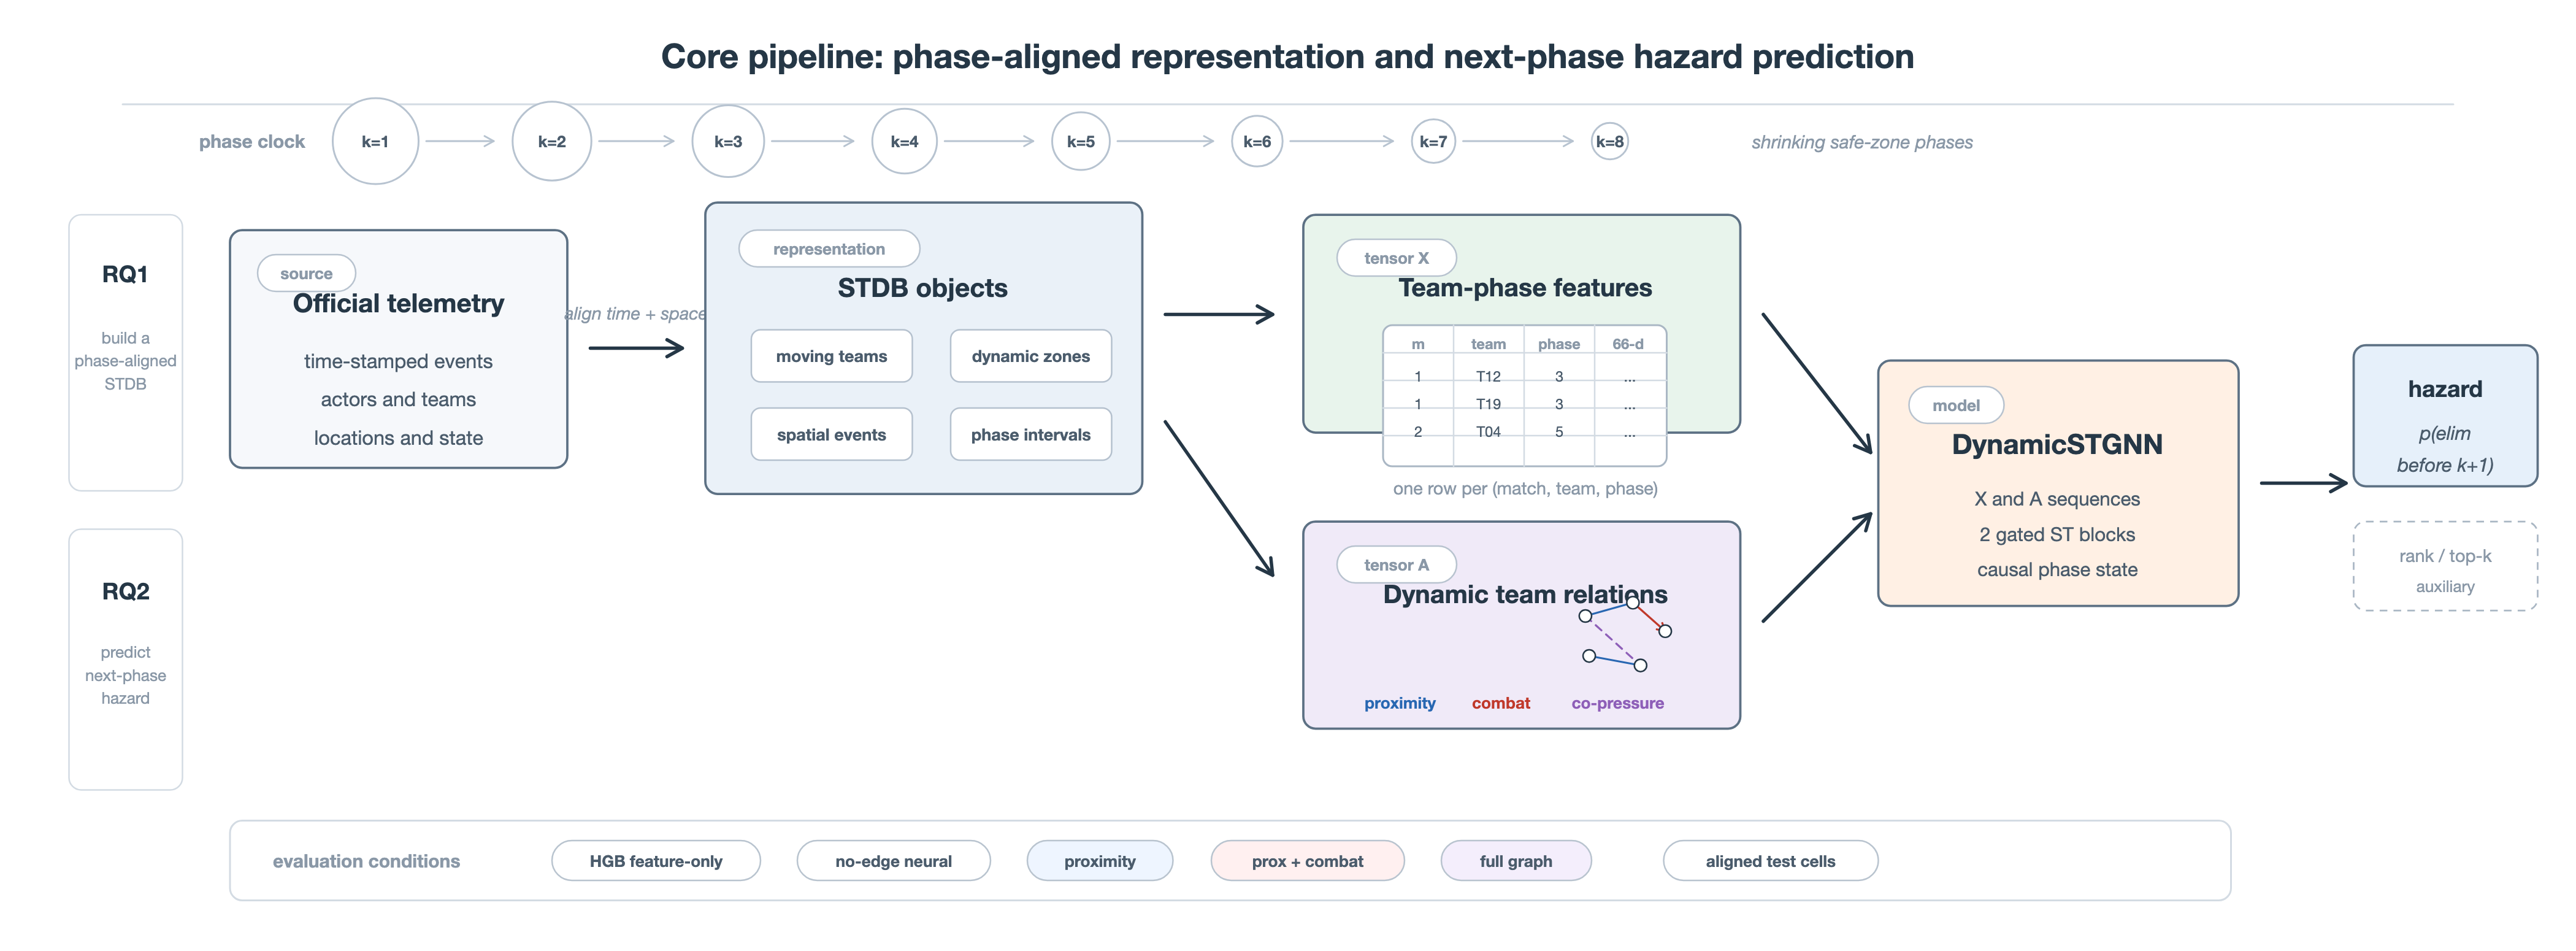
\includegraphics[width=0.86\textwidth]{figures/pipeline_overview.png}
\caption{Pipeline 개요. Official telemetry를 phase-정렬 STDB로 재구성하고
team-phase feature와 dynamic team graph로 요약한 뒤(RQ1), DynamicSTGNN을
feature-only model들과 비교해 next-phase elimination hazard를 평가한다(RQ2).}
\label{fig:pipeline-overview}
\end{figure*}

\begin{table}[t]
\centering
\caption{방법론 pipeline.}
\label{tab:rq-method-map}
\small
\begin{tabular}{p{0.12\linewidth}p{0.44\linewidth}p{0.30\linewidth}}
\toprule
RQ & 단계 & 산출물 \\
\midrule
RQ1 & Moving team, dynamic safe/blue zone, spatial event, phase interval을
STDB object로 표현한다. & Phase-aligned STDB. \\
RQ1 & 각 team의 trajectory, 구역 노출, 전투, 준비 상태를 phase 단위로
요약한다. & Team-phase feature row. \\
RQ1 & Phase별 팀 간 관계를 표현한다. & Dynamic team graph
\(G_1,\dots,G_T\). \\
RQ2-i & Feature row로 next-phase elimination hazard를 예측한다. & Hazard
task와 representation ablation. \\
RQ2-ii & Graph 관계가 추가 signal을 주는지 검증한다. & DynamicSTGNN과
edge ablation·통제 실험. \\
\bottomrule
\end{tabular}
\end{table}

\subsection{Phase-정렬 STDB 구성 (RQ1)}
\label{sec:methods-data}

본 연구는 공식 PUBG Developer API에서 match record를 수집한다
\cite{pubgDeveloperPortal,pubgTelemetryGuide}. Telemetry file은 time, actor,
location, game-state context를 가진 event stream이다
\cite{pubgTelemetryEvents,pubgTelemetryObjects}. 연구 모집단은 21,824개
match이며, 12개 map과 모든 표준 team mode---1인칭·3인칭의 solo, duo,
squad---를 포괄한다. 그중 3인칭 squad match가 가장 큰 비중(15,213)을
차지한다. 표~\ref{tab:api-fields}는 raw record를 어떻게 사용하는지 요약한다.

\begin{table*}[t]
\centering
\caption{Raw telemetry의 의미와 분석 표현.}
\label{tab:api-fields}
\small
\begin{tabular}{p{0.27\linewidth}p{0.31\linewidth}p{0.34\linewidth}}
\toprule
Raw information & Match 안에서의 의미 & 표현 \\
\midrule
Match 및 roster context & Map, mode, duration, team membership, outcome. &
Match/team record와 auxiliary placement target. \\
Timestamped player state & Location, health, alive status, vehicle state. &
Moving player, team centroid, state/movement feature. \\
시간에 따른 zone state & Safe-zone/blue-zone center, radius, timing. &
Dynamic region, phase interval, exposure feature. \\
Combat 및 elimination event & Attacker-victim interaction과 time, place,
damage context. & Spatial event, elimination time, combat relation. \\
Resource 및 support event & Equipment, resource use, healing, boosting. &
Team-phase readiness summary. \\
공통 time/location metadata & 분리된 record를 연결하는 coordinate. &
Trajectory, region, event, edge의 공통 축. \\
\bottomrule
\end{tabular}
\end{table*}

API는 event를 제공하지만 analysis object를 제공하지 않는다. 따라서 event
stream을 elapsed match time과 공통 map plane이라는 두 공유 축 위에서 네 가지
object type으로 변환한다. Player position은 10초 격자로 재표집된 뒤 team
centroid, 즉 moving object가 된다. Safe/blue-zone state는 phase-indexed
dynamic region이 된다. Combat과 elimination record는 특정 time과 place에
결합된 spatial event가 된다. Phase 경계는 명시적 interval
\([a_k,b_k]\)가 되며, 자기장 제시 전의 landing interval은 phase 0으로
indexing한다. 구체적으로 STDB는 표~\ref{tab:stdb-schema}의 relation
집합이며, team-phase feature·label·edge는 interval 집계---team state,
spatial event, zone geometry를 \([a_k,b_k]\)로 제한한 join---이다.

\begin{table}[t]
\centering
\caption{개념적 STDB schema. \(m\): match, \(i,j\): team, \(k\): phase,
\(t\): time, \(r\): relation type.}
\label{tab:stdb-schema}
\small
\begin{tabular}{llp{0.45\linewidth}}
\toprule
Relation & Key & 내용 \\
\midrule
Match & \(m\) & map, mode, duration \\
Team & \(m,i\) & roster 크기, outcome \\
Phase & \(m,k\) & interval \([a_k,b_k]\); safe/blue-zone geometry \\
Team state & \(m,i,t\) & centroid, 생존 인원, health, vehicle \\
Spatial event & \(m,e\) & time, place, attacker/victim team, kind, damage \\
Team-phase & \(m,i,k\) & 66 feature; hazard label \\
Edge & \(m,k,r,i,j\) & relation \(r\)의 weight \\
\bottomrule
\end{tabular}
\end{table}

표~\ref{tab:data-funnel}는 변환 funnel을 보고한다. 수집된 match와
graph-ready match 사이의 차이는 거의 전부 tutorial 및 training-range
session(5,658개)으로, 경쟁 플레이가 아니므로 설계상 제외한다. 그 외에는
위치 기록이 없거나 next-phase label을 정의할 phase가 부족한 비정상
telemetry로 인해 9개 match만이 추가로 제외된다.

\begin{table}[t]
\centering
\caption{Raw telemetry에서 graph-ready match까지의 data funnel.}
\label{tab:data-funnel}
\small
\begin{tabular}{lr}
\toprule
단계 & Matches \\
\midrule
Official telemetry retrieved & 27,491 \\
Converted to STDB & 21,833 \\
Team positions available & 21,830 \\
Team-phase features available & 21,830 \\
Next-phase labels available & 21,824 \\
Team-relation edges available & 21,830 \\
Graph-ready matches, \(N_{\max}=128\) & 21,824 \\
\bottomrule
\end{tabular}
\end{table}

\subsection{Team-Phase Feature (RQ1)}
\label{sec:methods-features}

모델링 단위는 team-phase tuple \((m,i,k)\), 즉 match \(m\), team \(i\),
phase \(k\)이다. 각 row는 한 phase 동안 한 team의 trajectory, 구역 노출,
전투, 준비 상태를 요약하며, row의 모든 수치는 해당 phase 안의 관측만으로
계산되고 phase의 종료 시점을 넘는 정보는 사용하지 않는다. Team 위치는 아직
탈락하지 않은 팀원들의 centroid,
\(c_{i,t}=|P_{i,t}|^{-1}\sum_{p\in P_{i,t}}\ell_{p,t}\)이다. 여기서
\(\ell_{p,t}\)는 player \(p\)의 위치이다. Centroid는 흩어진 squad를
단순화하므로, 같은 row에 team spread와 최근접 적 거리 feature를 두어 이를
보완한다. Zone에 상대적인 모든 수치(이동 정렬, zone 진입 시점, zone 밖
체류 시간)는 phase \(k\) 동안 이미 공개되어 플레이어가 관측 가능한 그
phase의 target safe zone을 기준으로 하며, 미래의 zone은 사용하지 않는다.
그림~\ref{fig:team-phase-feature-example}은 하나의 row가 담는 시점을
보여준다. Section~\ref{sec:related-work}의 habitat-contraction 관점에서
safe-zone 노출과 주변 팀 압박은 배경이 아니라 team risk state의 일부이다.

\begin{figure}[t]
\centering
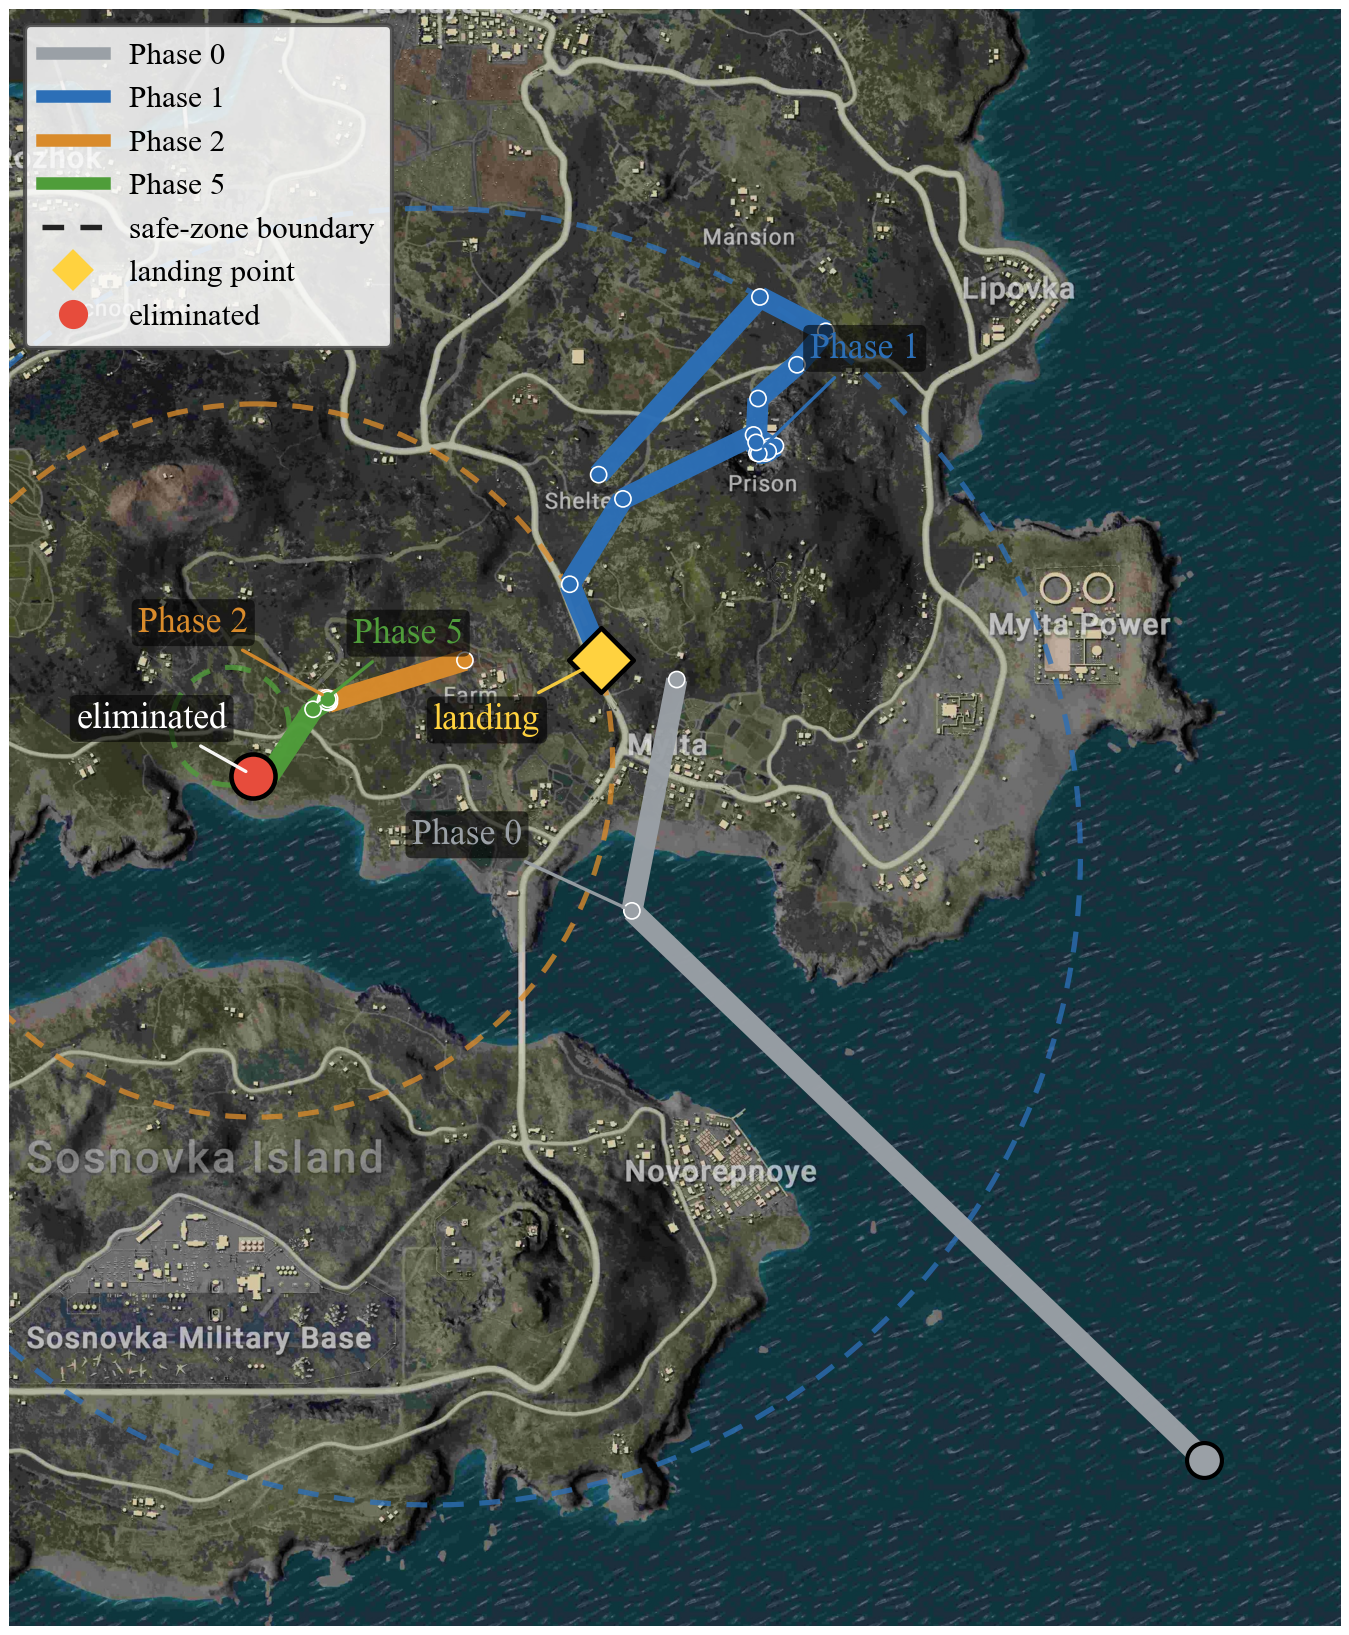
\includegraphics[width=0.48\textwidth]{figures/team_phase_feature_example.png}
\caption{시공간 과정으로서의 PUBG gameplay 예시. 실선은 선택된 phase에서 한
team의 centroid movement를 나타내며, 같은 색의 점선 원은 해당 phase의 target
safe-zone boundary를 Erangel 전장 위에 표시한다. Phase 0은 자기장 target이
제시되기 전의 landing interval을 의미하며, 노란 마름모는 landing point, 빨간
marker는 elimination을 나타낸다.}
\label{fig:team-phase-feature-example}
\end{figure}

표~\ref{tab:feature-groups}는 특징 원천을 기존 telemetry 집계와 본 연구에서
추가한 STDB 시공간 특징으로 구분한다. 66개 node feature 전체의 정의와
scaling은 Appendix~\ref{app:features}의 사전(dictionary)에 제시한다. 표의
\(d\)는 HGB 표현 ablation에 사용한 tabular 변수 수이며, DynamicSTGNN은 같은
원천을 정규화한 66차원 수치 vector를 node feature로 사용한다. STDB 단독
\(d=16\)에는 공통 phase index가 포함되고, 결합 표현에서는 이 중복 항목을
한 번만 센다. 각 수치는 특징별 고정 scale 상수로 나눈다. 피해량, item
획득, combat event 횟수처럼 드물게 큰 값이 나타나는 변수에는 log 압축을
적용한다. 이 scale은 training data에 적합(fit)한 통계량이 아니라 표현
자체의 상수이다.

\begin{table}[t]
\centering
\caption{기존 telemetry 집계와 추가 STDB 시공간 feature.}
\label{tab:feature-groups}
\scriptsize
\setlength{\tabcolsep}{2.5pt}
\begin{tabular}{p{0.18\linewidth}p{0.22\linewidth}rp{0.42\linewidth}}
\toprule
구분 & 특징군 & \(d\) & 대표 수치 \\
\midrule
기존 집계 & 페이즈/팀 상태, 교전, 준비도 & 57 &
페이즈 인덱스와 길이, 생존 팀/플레이어 수, 존 반경과 중심 이동, 체력,
팀 분산, 차량, 피해량, 기절, 처치, 아이템, 회복/부스트. \\
추가 STDB 시공간 & 궤적, 존/적 노출 & 16 &
팀 centroid 이동 거리, 순변위, 경로 굴곡도, 속도, 회전 시점, 안전 구역
방향 정렬과 진입 시점, 경계 거리, 블루존 밖 체류 비율, 주변 적 밀도,
최근접 적 거리, 교전 지역 통과. \\
결합 표현 & 기존+추가 STDB & 72 &
기존 집계에 STDB 궤적/노출 특징을 결합한 탈락 위험 예측용 tabular 표현. \\
\bottomrule
\end{tabular}
\end{table}

\subsection{Dynamic Team Graph (RQ1)}
\label{sec:team-graphs}

세 번째 표현 객체는 팀 간 관계를 명시적으로 만든다. Phase \(k\)에 대해 가중
이질 graph \(G_k=(V_k,X_k,\{A_k^r\}_{r\in R})\)를 정의한다. \(V_k\)는 함께
관측된 team의 집합, \(X_k\)는 절~\ref{sec:methods-features}의 team-phase
feature matrix, \(A_k^r\)는 relation \(r\)의 가중 adjacency
matrix이다~\cite{sanchezLengeling2021gnnIntro}. 따라서 하나의 match는 이산
시간 동적 graph가 된다. Phase마다 하나씩 만들어지는 snapshot의 sequence
\(G_1,\dots,G_T\)이며, team이 탈락하면 node도 빠진다. 모든 edge는 phase
\(k\)의 관측만으로 계산한다.

Relation set \(R\)는 세 channel로 구성된다.
\[
A^{\mathrm{prox}}_{ij,k}=e^{-\bar d_{ij,k}/\lambda},\qquad
A^{\mathrm{comb}}_{ij,k}=\log\!\big(1+D_{ij,k}+\gamma_e E_{ij,k}+\gamma_k K_{ij,k}\big),
\]
\[
A^{\mathrm{press}}_{ij,k}=\rho_{ij,k}\, e^{-\bar d^{\,\mathrm{p}}_{ij,k}/\lambda}.
\]
여기서 \(\bar d_{ij,k}\)는 phase 동안 두 team centroid 간 평균 거리,
\(D\)·\(E\)·\(K\)는 team \(i\)가 team \(j\)에게 가한 damage·elimination·
knockdown이다. Team이 safe zone 밖에 있거나 boundary로부터 \(\tau_b\) 이내이면
압박 상태로 정의하고, \(\rho_{ij,k}\)는 두 team이 서로 \(\tau_d\) 이내에서
함께 압박 상태로 보낸 phase 비율, \(\bar d^{\,\mathrm p}\)는 그 순간들의
평균 거리이다. Proximity는 대칭이며 완전(거리 컷오프 없음), co-pressure는
대칭이며 희소, combat은 방향성이며 희소하다. 상수는 map 규모에 맞춰 사전에
고정했다: \(\lambda=200\)\,m, \(\gamma_e=100\), \(\gamma_k=50\),
\(\tau_b=150\)\,m, \(\tau_d=200\)\,m. 이 값들은 조정하지 않았으며, 민감도는
한계에서 논의한다. Phase 1--8 평균으로 한 phase graph에는 약 14개 team이
함께 관측되며, phase당 평균 약 14개의 방향성 combat edge와 약 7개의
co-pressure pair가 있다.

각 channel은 team별 outgoing weight의 합이 1이 되도록 정규화한다:
\(\bar A^{r}_{ij,k}=A^{r}_{ij,k}/\sum_{j'}A^{r}_{ij',k}\). Edge가 없는 row는
0으로 남고, proximity channel에는 자기 자신의 feature를 보존하기 위한
self-loop를 두며, padding되었거나 탈락한 team은 어떤 edge도 갖지 않는다.
Model을 읽는 데 중요한 두 가지 관례가
있다. 첫째, combat은 attacker를 row로 저장한다. 집계 \(\bar A H\)에서
공격한 team이 자신이 damage를 가한 team들의 상태를 집계하며, 그 반대
신호---공격받음---는 node의 combat-taken feature가 운반한다. 둘째,
이 정규화는 team마다 연결 수가 달라도 graph aggregation의 규모가 과도하게
커지지 않도록 한다. 전투의 절대 강도는 node 수준 combat feature에
보존되므로, combat adjacency는 원시 크기가 아니라 교전 상대의 분포를
표현한다. 변환 과정은
그림~\ref{fig:dynamic-graph-example}에 예시한다.

\begin{figure*}[t]
\centering
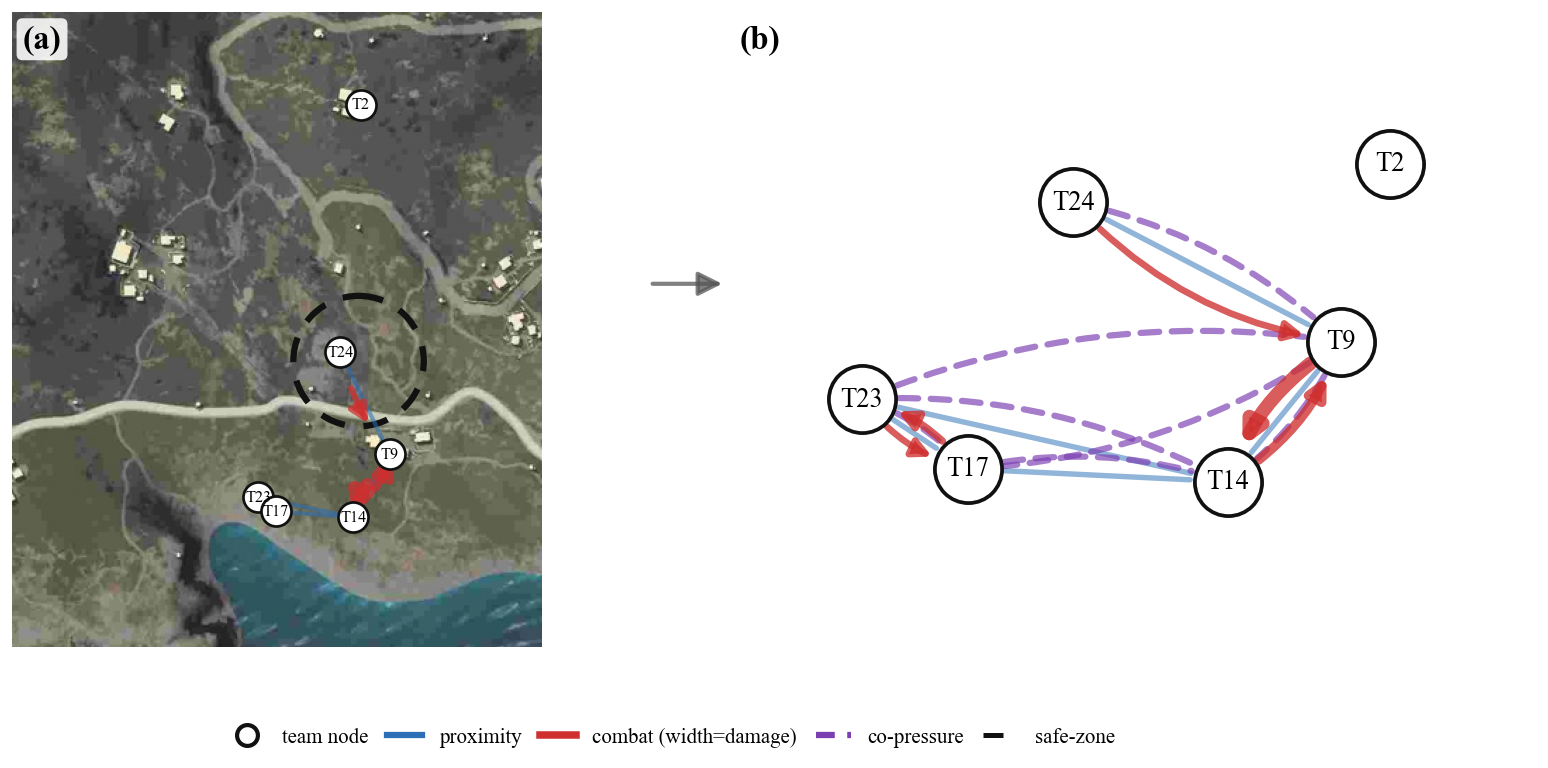
\includegraphics[width=0.86\textwidth]{figures/dynamic_heterogeneous_graph_example.png}
\caption{한 PUBG phase의 phase-level STDB snapshot을 dynamic team graph로
변환하는 시각적 예시. Panel (a)는 Erangel map 위의 team centroid, 현재 safe-zone
boundary, combat event를 보여준다. Panel (b)는 같은 team과 relation을 유지하되
map background를 제거하여 model이 사용하는 graph structure만 남긴 것이다.}
\label{fig:dynamic-graph-example}
\end{figure*}

이 설계에는 본 연구가 의존하는 네 가지 성질이 있다. 이질 channel은 서로
다른 위험 기제---어떤 team 곁에 있는 것, 그 team에게 공격당하는 것, 같은
축소 공간으로 함께 밀려나는 것---를 분리해 유지하고, 하나의 graph로
뭉개는 대신 model이 그 비중을 학습하게 한다. 컷오프 없는 완전 가중
proximity channel은 거리 임계값이라는 hyperparameter를 없애고 거리의 전체
순서 정보를 보존한다. Team이 밀집한 초반 phase에서는 과도한 smoothing의
위험이 있으나, 지수 감쇠가 가중치를 가까운 team에 집중시키고,
절~\ref{sec:dynamic-team-graph-model}의 no-edge·shuffle 통제가 무분별한
혼합에서 올 수 있는 이득의 상한을 제한한다. 방향성 combat edge는 누가
교전을 시작했는지를 유지한다. 마지막으로 snapshot 동역학은 graph의 시계를
hazard 과제의 phase 시계와 정렬하고, row normalization은 생존 team 수가
줄어들어도 이웃 집계의 규모를 비교 가능하게 유지한다.

\subsection{Next-Phase Hazard 예측 과제 (RQ2-i)}
\label{sec:prediction-task}

RQ2의 (i)는 절~\ref{sec:methods-features}의 feature만으로 next-phase 팀
탈락을 얼마나 정확히 예측할 수 있는지 묻는다. \(k\)를 \textit{cut phase}라고
부른다. Model은 phase \(k\)의 종료 시점까지만 match를 관측하고, team \(i\)가
phase \(k{+}1\) 동안 eliminated되는지 예측한다. 모든 입력---feature, edge,
mask---은 \(b_k\)까지 관측 가능한 telemetry만으로 구성하며, \(b_k\) 이후의
event와 outcome은 label 정의에만 사용한다.

\(b_k\)를 phase \(k\)의 종료 시점, \(T_i\)를 team \(i\)의 탈락 시점---마지막
생존 팀원이 제거되는 시점---이라고 하면 label과 hazard는 다음과 같다.
\[
Y_{i,k}=\Ind\!\left\{b_k < T_i \leq b_{k+1}\right\}, \qquad
h_{i,k}=P(b_k < T_i \leq b_{k+1}\mid T_i>b_k, X_{i,\leq k}).
\]
\(b_k\) 이전에 탈락한 team은 risk set에서 빠지며 mask된다. 생존한 team은
관측된 모든 interval에서 \(Y_{i,k}=0\)을 제공하지만, match가 종료되거나
8-phase horizon에 도달한 이후의 interval은 관측되지 않으므로 label을 주는
대신 right-censored로 처리한다. 모델링은 phase 1--8을 사용하고 landing
interval은 제외하므로 cut phase는 1부터 7까지이다. 학습은 mask된 이산 시간
생존 우도를 최소화한다.
\[
\mathcal{L}_{\mathrm{haz}}
= -\sum_{(m,i,k)\in \mathcal{R}}
\Big[ Y_{i,k}\log \hat h_{i,k} + (1-Y_{i,k})\log\big(1-\hat h_{i,k}\big) \Big].
\]
여기서 risk set \(\mathcal{R}\)는 \(T_i>b_k\)이고 다음 phase가 관측된
team-phase cell만을 포함하며, censored cell은 mask로 제외된다. Split은
row가 아니라 match 단위로만 수행한다. (i)에 대한 답은 두 방향으로 구한다.
Feature-only model의 절대 성능과, feature set을 선행연구식 strategy score
수준까지 축소해 가는 representation ablation이다(Experiments 절).

\subsection{DynamicSTGNN (RQ2-ii)}
\label{sec:dynamic-team-graph-model}

RQ2의 (ii)는 절~\ref{sec:team-graphs}의 dynamic team graph가 team-phase
feature를 넘어 추가 예측 signal을 제공하는지 묻는다. DynamicSTGNN은
\(X \in \mathbb{R}^{B \times T \times N \times F}\)와
\(A \in \mathbb{R}^{B \times T \times E \times N \times N}\)를 입력으로 받으며,
\(T{=}8\) phases, \(N_{\max}{=}128\) teams, \(F{=}66\) node features,
\(E{=}3\) relation channels를 사용한다. 전체 architecture는
그림~\ref{fig:dynstgnn-arch}에 제시한다. \(N_{\max}\)는 모든 mode의 최대
team 수(solo 최대 100)를 덮는 padding 크기이며, padding된 node는 edge를
갖지 않고 전 과정에서 mask된다. 입력 layer는 각 node를 64차원 state
\(H\)로 embedding하고, 동일한 spatio-temporal block 두 개가 이어진다. 각
block은 gated causal temporal convolution을 적용한 뒤, 다음의 heterogeneous
graph convolution을 적용한다.
\[
H' = \mathrm{ReLU}\Big(\sum_{r\in R} \alpha_r\, \bar{A}_k^r H W_r + H W_0\Big),
\qquad \alpha = \mathrm{softmax}(a).
\]
여기서 \(\bar{A}_k^r\)는 relation \(r\)의 row-normalize된 adjacency,
\(W_r\)와 \(W_0\)는 학습되는 projection, \(a\)는 학습되는 channel logit이다.
이어서 두 번째 gated causal temporal convolution을 적용하며, layer
normalization과 residual connection을 갖는다. Channel weight \(\alpha\)는
phase나 team에 조건화된 attention이 아니라 전역 scalar이다. 따라서 graph
module은 관계 channel이 추가 signal을 갖는지 검증하도록 설계된 것이지,
맥락 의존적인 관계 중요도를 모델링하려는 것이 아니다.

Tensor에는 \(T{=}8\)개의 slot이 있지만, model은 cut phase
\(k=1,\dots,7\)마다 하나의 hazard logit을 출력한다. Temporal convolution은
좌측 causal이고, layer normalization은 각 team-phase state의 feature 차원에
대해서만 적용되며(시간 축을 가로지르지 않음), padding된 phase와 탈락한
team은 message passing과 loss에서 mask된다. 작은 head가 각 team-phase
state를 절~\ref{sec:prediction-task}의 next-phase hazard logit으로 변환한다.
전체 model의 parameter는 약 0.34M이다.

\begin{figure*}[t]
\centering
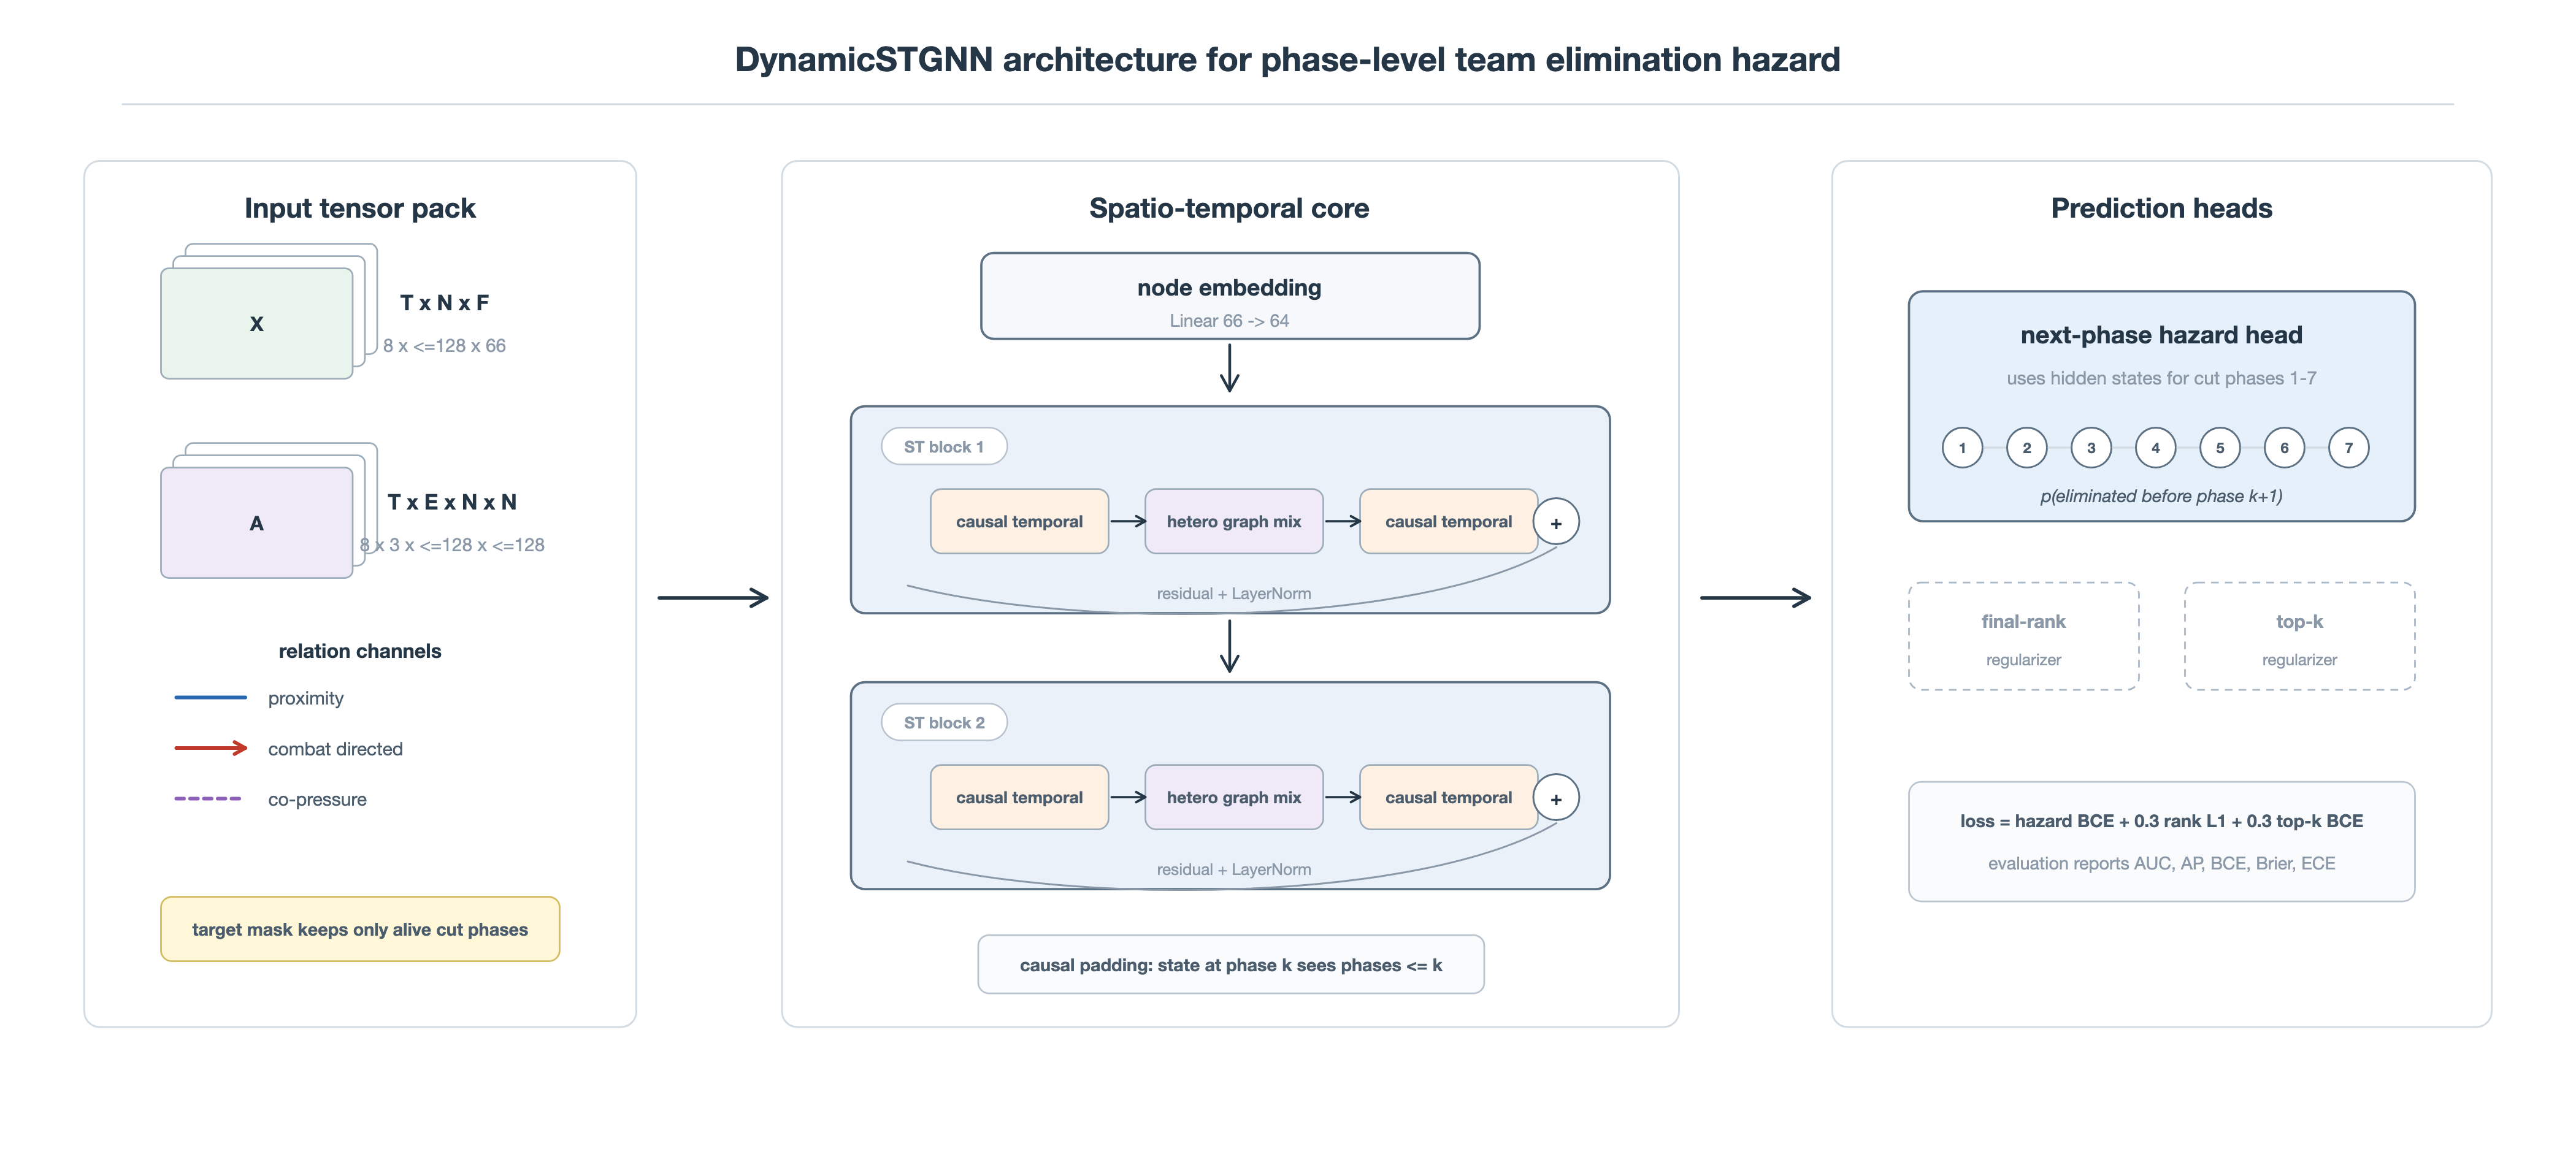
\includegraphics[width=0.86\textwidth]{figures/dynstgnn_architecture.png}
\caption{DynamicSTGNN. (a) 입력은 phase당 하나의 heterogeneous team
graph이며 proximity, combat, co-pressure 세 relation channel을 갖는다. (b)
Network는 node feature를 embedding한 뒤 gated spatio-temporal block 두 개를
쌓고 hazard head로 출력한다. (c) 각 ST block은 gated causal temporal convolution, relation channel별로 집계해
학습된 softmax weight와 skip connection으로 결합하는 heterogeneous graph
convolution, 두 번째 gated temporal convolution, 그리고 residual connection을
갖는 layer normalization을 적용한다. Causal padding은 phase \(k\)가 이후
phase를 보지 못하게 한다.}
\label{fig:dynstgnn-arch}
\end{figure*}

Ablation은 no edge, proximity only, proximity plus combat, full graph 네
조건을 비교한다. 또한 같은 team-phase row의 tabular view를 사용하는
histogram gradient boosting baseline과 비교한다. 두 기준 model의 역할은
구분된다. Boosting baseline은 graph model이 같은 표현 위의 강한 tabular
learner를 이기는지 검증하고, no-edge DynamicSTGNN은 관계 adjacency만 제거한
채 architecture, temporal convolution, parameter 수, multi-task
regularization을 통제한다. 두 기준 model 모두 node feature 안에 수작업
이웃 요약(주변 적 밀도, 최근접 적 거리)을 이미 받으므로, 이를 이긴다는
것은 그런 요약으로 포착되지 않는 관계 구조에 이득을 귀속시킨다. 두 기준을
모두 개선할 때에만 dynamic team relation의 signal을 주장한다. 이 결론은 두
가지 통제로 추가 검증한다. 이득이 정말 "누가 누구와 관계 맺는가"에서
온다면 추론 시 관측 graph 안에서 team identity를 섞었을 때 이득이 사라져야
하고, 학습을 서로 다른 random seed로 반복해도 이득이 유지되어야 한다.

